\section{Aufbau und Durchführung}
Der folgende Versuchsaufbau sowie die Durchführung basieren im Wesentlichen auf den Angaben in \cite{anleitungV01}.
\subsection{Aufbau}
\label{Aufbau}
Der Versuchsaufbau zur Bestimmung der Lebensdauer von Myonen ist in der \autoref{AufbauV01} abgebildet.
Der Aufbau umfasst einen Szintillatortankmit einem Volumen von ca. $50\,\unit{\litre}$, an dessen beiden Enden je ein Photomultiplier (PMT) montiert ist. Die Signale der PMTs werden über
Verzögerungsleitungen an Diskriminatoren mit einstellbarer Schwelle weitergeleitet. Die Pulsdauer am Ausgang dieser Diskriminatoren lässt sich ebenfalls
variieren. Die Ausgangssignale werden anschließen einer Koinzidenzschaltung zugeführt, die nur dann ein Signal erzeugt, wenn beide Pulse gleichzeitig anliegen.
Dieses Signal dient als Startimpuls für die nachfolgende Zeitmessung.\\
Das Koinzidenzsignal wird sowohl über zwei AND-Gattern als auch über eine zusätzliche Verzögerungsleitung von $30\,\unit{\nano\second}$ an ein Monoflop
weitergeleitet, das die maximale Suchzeit $T_S$ definiert. Die beiden AND-Gatter sind mit einem Time-Amplitude-Converter (TAC) verbunden, sodass eines die 
Zeitmessung beginnt, während das andere diese beendet. Über zusätzliche Leitungen, die mit einem Impulszähler verbunden sind, sit es möglich, die Anzahl der
Start- und Stoppimpulse zu erfassen. Durch eine geeignete Anordnung der Bauteile wird erreicht, dass die Zeitmessung startet, sobald ein Myon in das Detektionsvolumen
eintritt. Wenn das Myon zerfällt, wird die Zeitmessung gestoppt.\\
Das Signal des TAC wird anschließend an einen Vielkanalanalysator (MCA) weitergeleit, der über einen PC mit entsprechender Messsoftware ausgelesen wird. Außerdem steh 
für die Kalibrierung ein Doppelimpulsgenerator zur Verfügung, der bei $1\,\unit{\kilo\hertz}$ Doppelimpulse mit variablen Zeitabständen erzeugt.
\begin{figure}[H]
    \centering
    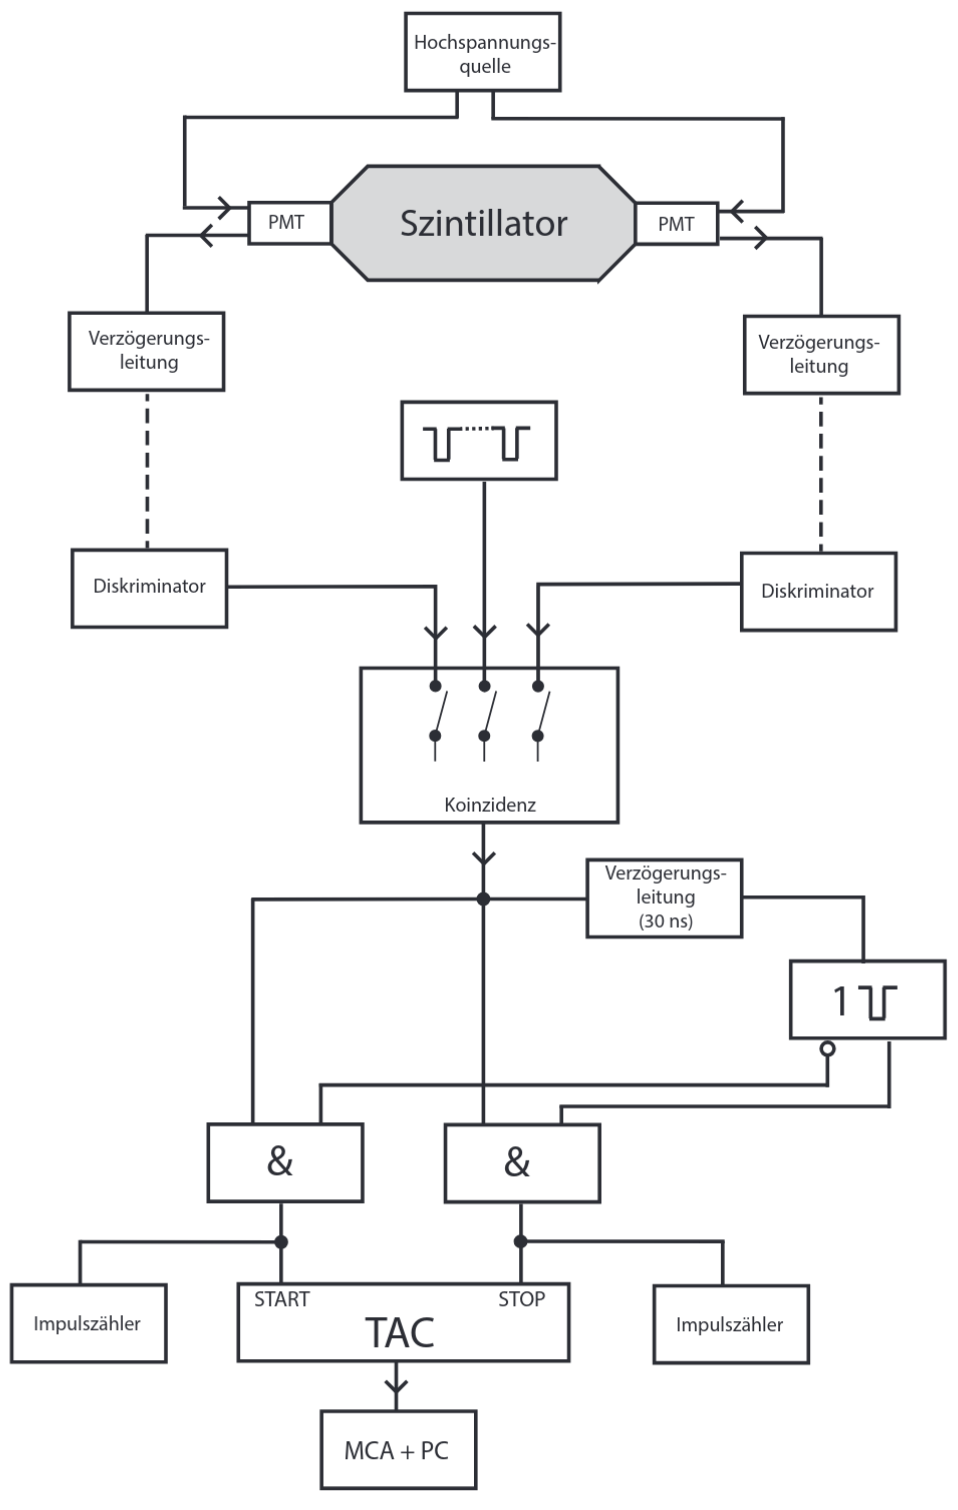
\includegraphics[width = 0.6\linewidth]{bilder/AufbauV01.png}
    \caption{Versuchsaufbau zur Bestimmung der Lebensdauer von Myonen. \cite{anleitungV01}}
    \label{AufbauV01}
\end{figure}
\subsection{Durchführung}
\label{sec:Durchführung}
Zunächst wird zur Kalibrierung des MCA ein Doppelimpulsgenerator angeschlossen. Mit diesem wird gemessen, welcher zeitliche Abstand zwischen zwei Impulsen welchem Kanal im 
MCA zugeordnet wird. Die Kalibrierung sollte mit mindestens zehn Messpunkten im Bereich von $0,3 - 9,9 \,\unit{\micro\second}$ durchgeführt werden. 
Um die Messgenauigkeit über den gesamten Bereich zu gewährleisten, sollte für alle Messpunkte die gleiche Messdauer einghalten werden. Hier wird die Messdauer von $30\,\unit{\second}$ gewählt.
Die Zählerraten können anschließend miteinander verglichen werden. Für den weitern Verlauf ist der Doppelimpulsgenerator nicht angeschlossen.\\
Sobald die Photomultiplier mit Hochspannung versorgt sind, sollten an ihren Ausgängen Spanungssingale mit unterschiedlichen Amplituden zu erkennen sein.
Dies kann mithilfe eines Oszilloskops überprüft werden.
Anschließend werden die Schwellenwerte der Diskriminatoren so eingestellt, dass an beiden Ausgängen etwa 30 Impulse pro Sekunde erzeugt werden. Dabei sollte eine
Pulsdauer von etwa $\Delta t = 10\,\unit{\nano\second}$ gewählt werden. Der Impulszähler hilft dabei, die Anzahl der Signale zu kontrollieren. Um die Koinzidenzschaltung richtig abzustimmen,
verändert man die Verzögerungsleitungen systematisch an beiden Pulse in dem Bereich $0-30\,\unit{\nano\second}$ und beobachtet die Veränderung der Impulsrate. Der gewählte Messbereich
ist dabei so groß, dass sich die Halbwertsbreite später zuverlässig bestimmen lässt. Nachdem eine geeignete Verzögerung gefunden wurde, bleibt diese für den gesamten Versuch unverändert.\\
Nach abgeschlossener Kalibrierung wird die Langzeitmessung zur Bestimmung der Lebensdauer gestartet, welche für mindestens $24\,\unit{\hour}$ durchgeführt wird.
